% chain-intersection.tex

\begin{tikzpicture}[node distance = 0.00cm]
  \node (abcd) [] {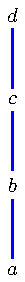
\includegraphics[scale = 0.30]{figs/chain-abcd}};
  \uncover<2->{\node (cap1) [red, right = of abcd] {$\cap$};}
  \node (acbd) [right = of cap1] {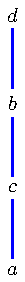
\includegraphics[scale = 0.30]{figs/chain-acbd}};
  \uncover<2->{\node (cap2) [red, right = of acbd] {$\cap$};}
  \node (acdb) [right = of cap2] {
\includegraphics[scale = 0.30]{figs/chain-acdb}};

  \node (eq) [purple, right = of acdb] {$=$};
  \node (poset-abcd-hasse-1) [right = of eq] {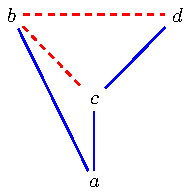
\includegraphics[scale = 0.40]{figs/poset-abcd-hasse-1}};
\end{tikzpicture}
